
\section{Rappel sur la géodynamique de l'atmosphère terrestre}%
\label{sec:structure_atmosphere}

\subsection{Composition chimique}%
\label{ssub:composition_chimique}

L'atmosphère de la terre est composée principalement de gas. Sa composition sèche est
faite d'diazote \ce{N2} à \SI{78.087}{\percent}, de dioxygène \ce{O2} à
\SI{20.95}{\percent}, argon \ce{Ar} à \SI{0.93}{\percent}. Parmis les pourcentages restant
se trouvent le dioxide de carbone \ce{CO2} (\SI{0.041}{\percent}) et le methane \ce{CH4},
en augmentation depuis le début de l'activité industrielle, ainsi que d'autres gas à
l'état de trace (néon \ce{Ne}, hélium \ce{He} et krypton \ce{Kr}).  Cette composition est
dite ''sèche'' car ne prend pas en compte la vapeur d'eau, représenant en moyenne 
\SI{0.25}{\percent} de la masse total de l'atmosphère, mais en quantité extrèmement
variable selon la localité géograhique ou temporelle.

De plus, sous l'effet des radiations solaire et notamment les longeurs d'ondes
ultra-violettes (UV), de nombreux radicaux hydroxyle \ce{HO^.} sont formés et réagissent
rapidement avec les autres composants de l'atmosphère.  La quantité de dioxygène et la
présence de radicaux hydroxyle, entre autre, font de l'atmosphère un milieu a grande
capacité oxydante ayant un impact directe sur les différentes réactions pouvant avoir lieu,
aussi bien avec les gas à effet de serre que pour les polluants organiques présent dans
les basses couches de l'atmosphère.

Enfin, il est à noté que l'atmosphère n'est pas composé que de gas mais également de
particule solide ou liquide en suspension, que ce soit des critaux de glace ou d'eau
liquide sous forme de nuage, mais également de ''poussières'', dont il sera question dans
cette thèse, et qui seront plus explicitement détaillé
ci-après~\ref{sec:les_aerosols_atmosphereiques}.

\subsection{Structuration de l'atmosphère}%
\label{sub:structuration_de_l_atmosphere}

\subsubsection{Une organisation stratifiée}%
\label{ssub:une_organisation_stratifiée}

À première vue l'atmosphère terrestre peut sembler homogène depuis le sol jusqu'à
l'espace. En réalité, de grande hétérogénéitées sont observées à certaines altitudes,
formant des couches concentriques aux propriétés physico-chimique très différentes, ne se
mélangeant que peu, limitant ainsi les échanges entre elles (voir
Figure~\ref{fig:chapter01/Comparison_US_standard_atmosphere_1962}).

Notamment, c'est dans la première strate atmosphérique, de \SI{0}{km} à \SI{13}{km} en
moyenne, la troposphère, que se déroule les phénomènes météorologiques
"directement sensible" au quotidien
(convection, formation de nuages, transport longue distance de poussières…).
C'est également la troposhère qui totalise près de \SI{75}{\percent} de la masse totale
de l'atmosphère, mais surtout en ce qui nous intéresse dans cette thèse, qui contient la
quasi totalité de l'eau et des aérosols.

La tropopause marque la séparation entre la troposhère et la stratosphère. Elle est
notable par son changement brutale de gradient thermique (\SI{-6}{\degreeCelsius\per\km}
dans la troposhère, à \SI{0}{\degreeCelsius\per\km} dans la bas de la stratosphère).
Ceci conduit à une inversion thermique très forte, faisant de la tropopause une véritable
barrière physique. La présence de la couche d'ozone (\ce{O3}) dans la stratosphère
protège la surface de la Terre d'une partie des UV provenant du soleil, en absorbant ces
radiations. Du fait de cette absorption par l'ozone, la stratosphère se réchauffe
progressivement avec l'altitude, jusqu'à arriver à une nouvelle frontière : la
stratopause, marquée par un gradient proche de 0.

Vient ensuite la mésosphère, dénuée d'ozone et présentant donc un refroidissement car au
contact du froid de l'espace. Puis la thermosphère, qui sous l'effet des radiations
solaires, formé des ions par photodissociation, réchauffe cette zone de l'atmosphère.
C'est également à cette altitude que se produissent les aurores-boréales, lorsque les
particules du vent solaire se heurtent au champs électromagnétique terrestre à environ
\SI{100}{km} d'altitude. Puis vient l'espace extra-terrestre après \SI{600}{km}
d'altitude.

\begin{figure}[ht]
    \centering
    \includegraphics[width=0.6\linewidth]{chapter01/Comparison_US_standard_atmosphere_1962.pdf}
    \caption{%
        Comparaison des variables atmosphèriques selon l'atmosphère standard défini par
        l'\textit{US standard atmosphere} de 1962.
        Source:
        \href{https://commons.wikimedia.org/wiki/File:Comparison_US_standard_atmosphere_1962.svg}{wikicommons},
        par \href{https://commons.wikimedia.org/wiki/User:Cmglee}{Cmglee}, CC-BY-SA.
    }%
    \label{fig:chapter01/Comparison_US_standard_atmosphere_1962}
\end{figure}

\subsubsection{La couche limite atmosphérique}%
\label{sub:la_couche_limite_atmospherique}

À l'interrieur de cette fine couche d'environ \SI{600}{km}, seule la troposhère,
c'est-à-dire les 13 premiers kilomètres, nous est directement familière. C'est en effet
dans la troposhère que les phénomènes météorologiques auquels nous sommes habitués s'y
déroulent : nuage, vent, pluie, etc. Alors que l'atmosphère parait immense, il est
important de noter la faible hauteur de cette couche.

La partie de la troposphère directement impactée par les effets de la surface terrestre
(friction, réchauffement, turbulence) est la couche limite atmosphèrique (CLA, ou
\textit{atmospheric boundary layer (ABL))}. Cette couche de quelques dizaines à centaines
de mètres, selons les lieux et période de la journée, a une dynamique rapide et
convective. En ce qui nous intéresse dans cette thèse, cela a pour conséquences que les
émissions de surface anthropiques ou naturelles, et notamment les polluants, seront
redistribués sur l'intégralité de cette hauteur.

Notamment, durant la nuit, la hauteur de la CLA est faible du fait de l'affaiblissement du
gradient thermique vertical lié à l'absence de réchauffement radiatif du sol (voir
Figure~\ref{fig:chapter01/Atmospheric_boundary_layer} et la mise en place de la couche de
surface après le couché du soleil). Après le levé du soleil, la surface se réchauffe et la
convection se met en place, rendant la CLA beaucoup plus homogène et diluant gaz et
particules dans un plus gros volume d'air. Les composés ne traverse cependant que
rarrement la couche d'inversion thermique, limite entre la CLA et la troposphère libre.
Ainsi, après le couché du soleil, on observe fréquement une couche résiduelle au milieu de
la CLA qui "capture" les composés d'une journée à une autre.

Il est à noter que des couches d'inversions thermiques à plus basse altitude peuvent se
mettre en place, notamment dans les vallées alpines. Pour un flux d'émission
constant, cela entrainne donc une accumulation forte des composés chimiques dans un volume
très restreint, augmentant mécaniquement les concentrations.
\textcite{allardQualite2018} a ainsi pu montrer que le gradient thermique est l'un facteur
explicatif les plus importants pour la compréhension de la compréhension des
concentrations en vallées alpines.
%Notamment, certains jours à Passy, France, un facteur de concentration de 700 était présent entre 

\begin{figure}[h]
    \centering
    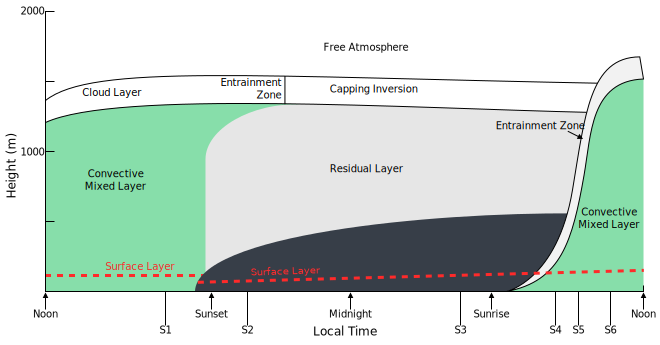
\includegraphics[width=0.8\linewidth]{chapter01/Atmospheric_boundary_layer.pdf}
    \caption{Évolution journalière schématique de la couche limite atmopshèrique.
        Credit: By
        \href{https://commons.wikimedia.org/w/index.php?curid=18862904}{NikNaks} - Own
        work based on:
        \url{http://ars.sciencedirect.com/content/image/1-s2.0-S0360128504000371-gr4.jpg}.
        See also: \url{http://www.archaeocosmology.org/eng/tropospherelayers.htm}., CC
        BY-SA 3.0
    }%
    \label{fig:chapter01/Atmospheric_boundary_layer}
\end{figure}

\section{Les aérosols atmospheriques}%
\label{sec:les_aerosols_atmosphereiques}

\subsection{Qu'est-ce qu'un aérosol ?}%
\label{sub:quest-ce-quun-aerosol}

L'air que nous respirons est constitué majoritairement de gas (\ce{N2}, \ce{O2},…) mais
également de particule solide ou liquide en suspension dans l'air. Ces particules, très
légères et de taille micrométriques ou moins, constituent une famille de composé appellé
communément particule fine, \textit{particulate matter} (PM) ou improprement particule
diesel dans le grand public.

Leur taille varient de quelques nanometres à plusieurs dizaines de micromètres.
À titre de comparaison, cela reviendrait à mettre dans la même catégorie une marche de
\SI{100}{m} pour aller chercher son pain à un voyage de \SI{10000}{km}.
Ainsi, cette nomenclature "PM" regroupe nécessairement des objets aux caractéristiques
très diverses. En effet, comme le montre la Figure~\ref{fig:aerosolDistribution}, selon
que l'on observe les PM en s'intéressant à leur nombre, surface ou volume, l'importance
relative des classes de tailles change complètement.
\begin{figure}[ht]
    \centering
    \includegraphics[width=0.5\textwidth]{aerosolDistribution.pdf}
    \caption{Distribution \textbf{(a)} en nombre, \textbf{(b)} surface, et
        \textbf{(c)} volume, pour un ensemble typique de distribution trimodale
        d'aérosols. Figure adaptée du livre de~\textcite{seinfieldAtmospheric1998}.}
    \label{fig:aerosolDistribution}
\end{figure}

La nomenclature des aérosols est ainsi historiquement fondé sur leur taille:
\begin{itemize}
    \item \PMdix, dont le diamètre aérodynamique inférieur ou égal à \SI{10}{\um}
    \item \PMdc, dont le diamètre aérodynamique inférieur ou égal à \SI{2.5}{\um}
    \item \PMun, dont le diamètre aérodynamique inférieur ou égal à \SI{1}{\um}
\end{itemize}

Ces différents modes reflètes différents procédés conduisant à leur présence dans l'air,
allant de la nucléation à partir de composé gaseux ou de source de combustion pour le mode
dit d'Aikten, le plus fins (prépondérant en nombre), permettant par coagulation
d'atteindre des particules plus grosses (mode d'accumulation) allant jusqu'au \PMdc, pour
enfin, lorsque la vitesse de coagulation est suffisante, atteindre le mode grossier
\PMdix, pouvant également être allimenté par diverse autres sources comme la remise en
suspension par le vent, les pollens, les activités humaines, etc, comme nous le verons
plus loin.

These categories do not have the same
chemical composition nor shape as they reflect different source or different process in
place in the atmosphere. Indeed, aerosols can react with the gas (\ce{SO2},
\ce{NO2}, \ce{NH3} for instance), radiation or radicals (the so call hydroxyl radical
\ce{HO^.}) or even with other aerosols and form new species or bigger aerosols. We then
call this aerosol \emph{secondary aerosol} as it do not reflect a primary source but
reaction in the atmosphere.

\begin{figure}[ht]
    \centering
    \includegraphics[width=1.0\textwidth]{aerosol_micrographs.jpg}
    \caption{Image au microscope electronique à balayage, à des échelles différentes,
        illustrant la diversité de forme des aérosols.
        De gauche à droite : cendre volcanic, polen, sel de mer et suie. Micrographies de
        l'USGS, UMBC (Chere Petty) et de l'Arizona State University (Peter Buseck). Credit
        : NASA earthobservatory
    \url{https://earthobservatory.nasa.gov/Features/Aerosols/}.}
    \label{fig:micrography}
\end{figure}
An aerosol is composed of several chemical species like ions (\SOq, \NOt, \ce{Na+},
\ce{Cl-}, \ce{Mg^2+}, etc), metals (\ce{Cu}, \ce{Al}, \ce{Ti}, \ce{Ca}, etc), and organics species
(cellulose or other sugar, \og black carbon\fg, hopanes, etc).  They come from different
sources: natural like volcano, biology, desert (resuspension due to the wind) or marine
spray for instance and anthropogenic like traffic exhaust, brake wear, industry, biomass
burning or agriculture.  Each of these sources emits different species, in different
quantity and in different place of the atmosphere and of the Earth and with different
shape as shown in fig.~\ref{fig:micrography}.  However, the average lifetime of an aerosol
is from hour to week, and then can impact a wide area.  For instance the black carbon
emitted in developed countries is a major issue for the ice melt in the Artic's iceshelf.
More generally, aerosols are a key parameter in the climate system as they interact with
the Solar and Earth radiation, act as cloud/ice condensation nucleii and sectionicipate to
the precipitation process \autocite{boucherClouds2013}.


\subsection{Impacts climatiques des aérosols}%
\label{sub:impacts_climatiques_des_aerosols}
\paragraph{Noyaux de condensation}%
\label{par:noyaux_de_condensation}

\paragraph{Impact radiatif}%
\label{par:impact_radiatif}



\subsection{Impacts environnementaux}%
\label{sub:impacts_environnementaux}

\paragraph{Transport longue distance}%
\label{par:transport_longue_distance}


\paragraph{Polluants émergents}%
\label{par:polluants_emergents}



\subsection{Impacts sanitaires}%
\label{sub:impacts_sanitaires}



\section{Détermination des sources d'émission des PM}%
\label{sec:source_apportionment_of_pm}

\subsection{Signature chimique des sources d'émissions}%
\label{sec:chemical_signature_of_the_sources}

\subsection{Source apportionment model}%
\label{sec:source_apportionment_model}

\subsubsection{Direct modeling}%
\label{sub:direct_modeling}

\paragraph{Lagrangian or dispersion model}%
\label{sub:lagrangian_or_dispersion_model}

\paragraph{Deterministic chemistry transport model (CTM)}%
\label{sub:deterministic_chemistry_transport_model_ctm_}

\subsubsection{Receptor model}%
\label{sec:receptor_model}

\paragraph{Chemical mass balance (CMB)}%
\label{sub:chemical_mass_balance_cmb_}

\paragraph{Principal component analysis (PCA)}%
\label{sub:principal_component_analysis_pca_}

\paragraph{Positive matrix factorization (PMF)}%
\label{sub:positive_matrix_factorization_pmf_}


\section{Vers une mesure unifiée: le potentiel oxydant}%
\label{sec:le_potentiel_oxydant_des_aerosols}

Devant la grande variété de chimie, forme, taille, etc. des aérosols, il apparaît
compliqué de résumer la toxicité de l'air que l'on respire à sa simple concentration
massique en aérosols. En effet, il est évident que respirer un~\ugm{} de sable n'aura pas
le même impact sur notre santé qu'un~\ugm{} de mercure ou de plomb.
Seulement, la mesure massique est l'une des plus simples a implémenter en routine et est
également facilement automatisable, permettant ainsi un premier ordre de grandeur de 
l'exposition des populations. Aussi, il est important de rappeler que les aérosols n'ont
pas qu'un impacte sanitaire, mais également climatique (voir
section~\ref{sub:impacts_climatiques_des_aerosols}), pour lequel la messure de la concentration est tout a
fait adaptée.

Afin de répondre à ce problème, il a été proposé dans les années 2010 une nouvelle mesure,
intégratrice des propriétés physico-chimique des aérosols, sensé être plus proche des
impacte sanitaire occasioné par les PM. En effet, un des mécanismes suspecté d'être à
l'origine des troubles sanitaires engendrés par les aérosols est le stresse oxydatif
induit lors de l'inhalation des particules, entrainant une cascade de réaction au sain de
notre organisme.
Cette nouvelle mesure tente de quantifier les espèces réactive de l'oxygène (ROS) présente
ou induite par les aérosols en mettant en contact les aérosols et un antioxydant.
Le suivit de la cinétique de la réaction permet ainsi d'estimer la réactivité de la
particule, prenant en compte non seulement sa chimie, mais aussi la taille et forme des
particules à travers leurs surface de réaction et également les potentiels "effet
cocktail" lors de la combinaison de différentes espèces chimiques.

\subsection{Methodologie de mesure}%
\label{sub:methodologie_de_mesure}

\subsubsection{Prendre en compte la bioaccessibilité: SLF}%
\label{sub:prendre_en_compte_la_bioaccessibilite_slf}

\subsubsection{Differents agent réactant}%
\label{ssub:differents_agent_reactant}

\paragraph{Mesure par Ditiothreitol}%
\label{ssub:mesure_par_ditiothreitol}

\paragraph{Mesure par Acide ascorbic}%
\label{ssub:mesure_par_acide_ascorbic}

\paragraph{Mesure par DCFH}%
\label{ssub:mesure_par_dcfh}

\paragraph{Autres methodes de mesure}%
\label{sub:autres_methodes_de_mesure}

\subsubsection{Unitées de mesures}%
\label{ssub:unitees_de_mesures}

Mesure de réactivité par ug de PM ou par m3 d'air respirer.

\subsection{État de la connaissance du PO}%
\label{sub:etat_de_la_connaissance_du_po}



\addcontentsline{toc}{section}{Bibliography}
\printbibliography[segment=2,heading=subbibliography]
